%!TEX root = ../PhDthesis.tex
\chapter{Modeling the effects of visual statistics on long-range lateral connectivity in visual cortex}

One of the major problems in computational neuroscience is in
understanding how the brain can robustly capture information about its
environment to improve how new information is encoded and
processed. One of the major strengths of developmental models such
as those developed in the previous chapters is that the developed
synaptic connections reflect the visual statistics of the
input. Therefore we can make predictions about how the statistics
embedded in the visual inputs will be reflected in the organization of the
model and could be used to aid cortical computations.

A number of studies have investigated the role visual statistics play
in shaping the organization of cortex. In particular it has been shown
that the distribution of orientations in the orientation maps can be
strongly affected by altering the visual experience of an animal
through manipulations like goggle rearing \citep{Tanaka2006}. However,
the evidence for the encoding of second-order statistics in lateral
connections has been much harder to study, and even coarse approaches
such as measuring the isotropy of lateral connections along the axis
of preferred orientation has not yielded uniform results. While a
number of studies have found that lateral connections are elongated
along the axis of preferred orientation in tree shrew
\citep{Bosking1997}, cat \citep{Schmidt1997}, and owl monkey
\citep{Sincich2001}, in macaque this anisotropy may simply be explained by
the anisotropy in cortical magnification such that the connections are
not actually elongated in visual space \citep{Angelucci2002}.  Whether
the different results reported per species are truly species
differences or simply differences between the various laboratories and
rearing environments involved is not fully clear. Unfortunately, the
tracer injections required to reconstruct the lateral connections can
be performed at most on a few cells in a single animal, making
systematic collection of comprehensive data infeasible.

Although there is a clear lack of data in this area, a few attempts
have been made to go further and establish whether the lateral
projections connect co-circular orientation domains, reflecting the
co-circularity in natural images \citep{Hunt2011}. These studies have
again been inconclusive due to the sparsity of clear data.

In this chapter, we will employ the model introduced in the previous
chapter to analyze to what extent the detailed statistics of the
visual input shape the long-range excitatory connections.  In
particular, we will attempt to reconstruct those statistics based
purely on synaptic weights and the orientation map. In doing so we
will determine to what extent the network has captured the statistics
of the training dataset, and establish whether considerable biases in
the inputs could affect the isotropy of connections.

\section{Methods}

We will first introduce the methods for computing comparable
statistics for natural images and for the LESPI network, which we can
use to analyze how well the network has extracted the underlying
patterns in the training data.

\subsection{Co-occurence statistics}

Natural image statistics have been well
characterized in a number of papers. For instance, 
\cite{Perrinet2015} analyzed the edge co-occurence statistics in
natural images by labeling images with edges at varying frequencies,
scales, orientations, and phases through a greedy algorithm, and then
computed both the relative orientation between each pair of edges, and
the normalized azimuthal angle between them. An example image with
labeled edges is shown in Figure~\ref{classifier}, along with a
diagram showing how the co-occurences were computed. Similar analysis
approaches have been used to visualize the co-occurrence statistics in
natural images, such as those produced by \cite{Geisler2001} to
predict the performance of human subjects in contour-detection tasks.

\begin{figure}
	\centering
    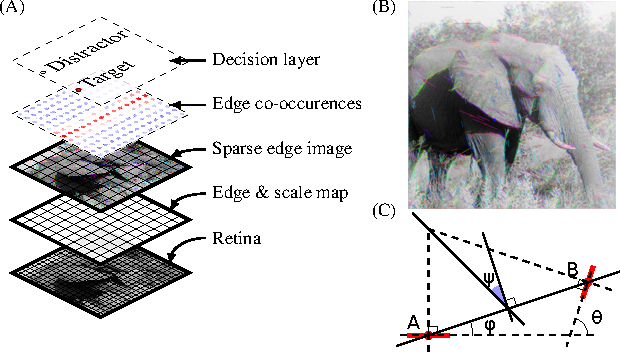
\includegraphics[width=0.8\textwidth]{./classifier.pdf}
	\caption[] {Diagrammatic representation of how a classifier is
      trained to distinguish between natural images and inanimate
      objects. A) The different layers used to train the
      classifier. The natural images are first fed through a model
      retina, all the edges are labeled with positions and
      scales. Using a greedy algorithm a set of edges accounting for
      the largest amount of luminance variance within the original
      image are selected. Using this set of edges the edge
      co-occurence statistics were computed and finally the classifier
      was trained based on these statistics. B) The sparse set
      of labeled edges extracted from a single image. C) Diagram
      showing how the angular difference $\theta$ and azimuth angle
      $\phi$ and relative azimuth $\psi$ are computed from two
      edges. Reproduced from \cite{Perrinet2015}.}
	\label{classifier}
\end{figure}

The afferent receptive fields in the visual cortex are usually assumed
to act as feature detectors (or at least feature-selective units),
reducing the dimensionality of the visual 
``pixel'' space into a lower-dimensional representation. Connections
between these feature detectors could therefore at least in theory
represent the co-occurence statistics of the low-level features. In
primary visual cortex they could therefore represent the co-occurence
of simple oriented edges. In order to test this idea, the models
were trained on various synthetic and natural image datasets, and the
statistics embedded in the lateral connections were decoded.

This analysis was done by computing the angles $\theta$, $\phi$, and $\psi$ (as
defined in figure (C) in Figure~\ref{classifier}) as well as the
Euclidean distance of the receptive-field centers for each pre- and
post-synaptic pair of neurons and then binning them weighted by the
strength of connections between them. The angle $\theta$ was computed
simply as the difference between the pre- and post-synaptic neurons'
orientation preference in the orientation map, and the position was
defined by computing the center of gravity of the neuron's afferent receptive
fields, allowing the angles $\phi$ and $\psi$ to be calculated. As in
the previous chapter, the weights were first thresholded, leaving only the
strongest 10\% to ensure that the model roughly matches the known
sparse and patchy pattern observed in anatomical tracing
studies. Additionally, neurons were selected from strong
iso-orientation regions by selecting the neurons with a local
homogeneity index above the 50th percentile, to mirror the procedure
of \cite{Bosking1997}. The resulting histograms and lateral connection
plots could then be further analyzed.

\subsubsection*{Univariate statistics}

The simplest way to analyze these statistics is to collapse across
the dimensions to visualize the univariate distributions of the
$\theta$, $\phi$, and distance of connections. This procedure provides
(1) an easily understood analysis to demonstrate how strongly the
connections are biased for similar orientations and co-linear
directions, (2) an indication of how isotropic the lateral connections
are in the model, and finally (3) the distances.

\subsubsection*{Multi-variate statistics}

Using the computed histogram, various plots can be generated to
compare against the plots produced by directly extracting the edge
co-occurrences from images in the \cite{Perrinet2015} and
\cite{Geisler2001} studies.

The first of these plots (Figure~\ref{SyntheticCooccurrence}), called
a ``chevron map'', presents the bivariate distribution of $\theta$ and
$\psi$, highlighting which spatial arrangement of edges is most likely
to co-occur. In these plots, the central $1^\circ$ diameter region of
the lateral field was ignored so the plot would reflect co-occurrence
statistics of connections \emph{outside} the receptive field of the
neuron. This procedure also allowed comparing the co-occurrences between
datasets by taking the ratio of normalized weights in each bins.

The \cite{Geisler2001} type of co-occurence plots, on the other hand,
reflect three dimensions, the angles $\theta$ and $\phi$ and the
distance, displaying the probability of an edge of a particular
orientation, co-occurring at a particular distance and azimuth
relative to the edge. It is then possible to plot the data to ask
two related questions: (1) what is the most likely orientation of an
edge given the distance and azimuth, and (2) where is the most likely
position of an edge of a specific orientation at a specific
distance. These will be referred to as the co-circularity and
co-linearity maps respectively. \cite{Geisler2001} asked humans to analyze
natural image patterns for this analysis, providing a direct measure
of the statistics. In the model there is only the weights, from which we can
decode the statistics. In addition to taking the weight to
compute each co-occurrence, the selectivity for each orientation and
azimuth were also determined by computing the vector sum.

\subsubsection*{von Mises Model}

Finally, the lateral weights were again fit using the von Mises model
with both Gaussian and orientation-preference--dependent components,
which was first introduced in Section~\ref{BuzasEquations}. This procedure
allows us to provide a quantitative assessment of how well the lateral
connections can be approximated with a simple model that is made up of
orientation, direction, and spatially dependent components. Most
importantly, the direction-dependent component allows us to quantify
how strongly the lateral connection fields are biased along the axis
of preferred orientation, a key issue from the literature.

\subsection{Training stimuli}
\label{synthetic}

Because natural images introduce a variety of RF shapes and phases,
not just long-range correlations, we will first look at the results
from synthetic stimuli constructed to have long-range correlations.
%%
These stimuli are simple extensions of the
elongated 2D Gaussian stimuli used to train the SCAL and SEPI models.
The model will draw 1 pattern per unit area of simulated model, which consists of
a chain of three Gaussian patterns (see
Figure~\ref{GaussianStatistics}). The middle Gaussian determines the
overall orientation ($\theta_M$) of the pattern, and the outer
Gaussians are offset in orientation by a value drawn from a von Mises
distribution with a mean of $\theta_M$ and a $\kappa$ of either $0.5$
or $8$. The patterns are then spatially offset so that they form a
chain forming an `S' shape. By varying the $\kappa$ we can vary how
the distribution of co-occurence statistics affects the preference
for simple elongated bars.

\begin{figure}
	\centering
	\includegraphics[width=1.0\textwidth]{./results/lespi/gaussian_statistics.pdf}
	\caption[Example of Gaussian patterns with co-occurence
      statistics] {Gaussian patterns with co-occurence statistics
      where the orientation offset is drawn from a von Mises
      distribution with different $\kappa$ values changing the
      distribution of orientation offsets.}
    \label{GaussianStatistics}
\end{figure}

We will also train the model on two natural-image datasets that had
previously been analyzed for their co-occurence statistics
(\citealt{Perrinet2015}; see Figure~\ref{classifier}), plus an
additional image dataset recorded in 2010 in juvenile tree-shrew cages
in David Fitzpatrick's lab at Duke University.  The tree-shrew cage
images feature great numbers of highly extended, high-contrast bars
(shown in figure \ref{image_patterns}), and are examples of the
rearing environment for the animals in the \cite{Bosking1997} study.
Thus the statistics of these patterns could be what the
\cite{Bosking1997} tree shrews encoded in their visual cortex, if the
hypotheses from this chapter are valid.

\section{Results}

We will start with the synthetic-stimulus--trained model, to ensure
the approaches work well in the simple case, which we will then extend
to the more complex natural-image--trained models.

\subsection{Synthetic Stimuli}

The stimuli described in Section \ref{synthetic} vary in both relative
orientation and azimuth, which means that if the lateral connections
capture the correlations in the inputs, then these correlations should
also be captured and vary depending on the width of the von Mises
distributions the orientation offsets are drawn from.

\begin{figure}
	\centering
    \includegraphics[width=1.0\textwidth]{./results/lespi/Synthetic_Distributions.pdf}
	\caption[Distributions of lateral connections of models trained on
      synthetic stimuli]{Lateral connections and histograms describing
      their orientation, azimuth and distance dependent distributions
      for narrowly and widely distributed synthetic stimuli. A, B)
      Example lateral excitatory weights after thresholding for the
      widely distributed ($\kappa=0.5$) and narrowly distributed
      ($\kappa=8$) condition. C) Orientation distribution of lateral
      connections, showing stronger bias for iso-orientations in the
      narrowly distributed condition. D) Azimuth distribution, showing
      strong co-linear bias for both conditions. E) Distance
      distribution, showing more weight at distant locations in the
      narrowly distributed condition.}
	\label{SyntheticDistributions}
\end{figure}

By analyzing and binning the lateral weights by orientation
difference, relative azimuth and distance we can get begin to
understand what the lateral connections are actually capturing. The
difference in lateral fields between a model trained on the synthetic
stimuli with a very wide distribution ($\kappa=0.5$) and a much
tighter distribution ($\kappa=8$) is shown in
Figure~\ref{SyntheticDistributions}. This simple analysis already
makes it clear that both conditions show a strong preference for
similar orientations and co-linear stimuli, as can be seen when
looking at the azimuth histogram, which highlights a strong isotropy
along the axis of preferred orientation. This can indeed be seen even
when just looking at the sample lateral connection fields directly
(Figure~\ref{SyntheticDistributions}A,B). The analysis also highlights
that the model trained on patterns drawn from the tighter distribution
has a slightly stronger preference for similar orientations, and more
weights at larger distances. This reflects the stronger bias for long
iso-oriented and co-linear contours in the input patterns.

\begin{figure}
	\centering
        \includegraphics[width=1.0\textwidth]{./results/lespi/Synthetic_Cooccurrences.pdf}
	\caption[Chevron map showing the distribution of orientation and
      azimuth differences between pre- and post-synaptic
      neurons.]{Chevron map showing the distribution of orientation
      and azimuth differences between pre- and post-synaptic neurons
      weighted by connection strength for the wide distribution
      (left), narrow distribution (middle), and the difference between
      them (right). Modeled after the \cite{Perrinet2015}
      co-occurrence analysis of natural images. Each `chevron`
      represents one particular configuration of two edges, varying by
      $\psi$ (relative azimuth) along the x-axis and $\theta$
      (orientation difference) along the y-axis. Increased probability
      is shown in red, and lower probabilities shown in blue. These
      results highlight the stronger bias for connecting
      iso-orientation regions in the model trained on narrowly
      distributed synthetic patterns.}
	\label{SyntheticCooccurrence}
\end{figure}

The chevron map of edge co-occurrences in
Figure~\ref{SyntheticCooccurrence} highlights very similar trends. In
particular it demonstrates a greater spread in co-occurring
orientations as the distribution of orientation offsets in the input
pattern widens. Both the azimuth distribution and the co-occurrence
histogram also emphasize an increased preference of parallel alignment
for the tighter distribution. It is not quite clear what drives these
correlations, but through parameter exploration not shown here it was
determined that they could be reduced by presenting fewer overlapping
patterns, suggesting that they were due to increased likelihood of
chance alignments.

\begin{figure}
	\centering
    \includegraphics[width=1.0\textwidth]{./results/lespi/Geisler_Synthetic_Cooccurrence.pdf}
	\caption{Co-occurrence statistics extracted from lateral
      connections to highlight the most likely orientation at each
      distance and azimuth for the two conditions (top row) and the
      most likely azimuth for each orientation and distance (bottom
      row). The colormap represents the relative probability of each
      configuration, while the size reflects the selectivity for that
      particular arrangement. The more narrow distribution ($\kappa$)
      results in more weight at the furthest distances and greater
      confidence in co-circular arrangements, however in both
      conditions co-linearity and co-circularity are decoded almost
      perfectly. }
	\label{SyntheticGeisler}
\end{figure}

A further analysis using plots originally developed by
\cite{Geisler2001} demonstrates just how well the network has captured
the co-occurrence statistics of the input. The co-linearity plot
almost perfectly reflects the statistics of the input, in that the
same orientation is encountered along the axis of preferred
orientation and as we move away from this axis the preferred angle
slowly shifts away from this orientation, which is precisely how the
input pattern is defined. The model trained on the dataset with a
narrower distribution also exhibits a narrower distribution in the
co-circularity plots. This means the model has captured not just the
rough characteristics of the input but also some subtle relationships
that are not immediately obvious. Even so, the statistics of the
synthetic training patterns are very simplistic, and capturing the far
broader distribution of visual statistics, including spatial
frequencies and spatial arrangements of patterns that are present in
natural images is a more difficult task.

\subsection{Natural Images}

Natural and man-made environments have very different statistics,
which may be reflected in the lateral connections in the primary
visual cortex. So far we have seen that the LESPI model can indeed
capture the statistics of a simplified input pattern. Now we will
train the model on a number of different image datasets, either from
natural environments or artificial structures such as laboratory
environments in which animals are raised. Using detailed labeling and
analysis of these datasets, which include those used by
\cite{Perrinet2015} and \cite{Serre2007}, we will demonstrate that the
lateral connections in V1 can already capture the differences between
different datasets.  We will suggest that the rearing environment of
an animal can have strong effects on the organization of the visual
system, which should be considered when using animal models.

Man-made environments are characterized by co-linear, parallel, and
orthogonal arrangements of edges, while true natural images, i.e.,
images of natural environments, exhibit more curvature and textured
patterns \citep{Perrinet2015}. In order to test whether the model
would capture these differences, three natural-image datasets were
used: (1) the ``natural`` dataset containing a lot of grass textures,
(2) the ``treeshrew`` laboratory cage containing long, high contrast
bars, and (3) the \cite{Serre2007} target dataset of natural scenes
and animals. These represent three highly distinct visual
environments, which should be reflected in long range connections.

\subsubsection*{First-order statistics}

Before investigating more complex second-order statistics, we analyzed
whether particular orientations were hugely overrepresented in the
orientation map, which could introduce systematic biases to the
results. As can be seen in Figure~\ref{NatImgORs}, both datasets show
some bias for specific orientations, with the tree shrew condition
exhibiting a stronger bias along the horizontal and vertical
axes. These biases are likely an artifact arising from the artificial
border at the edge of the simulated sheet, which can affect the whole
map through long-range interactions.

% jbednar: change 'natural' to 'outdoor' throughout if possible;
% natural is just so vague!
\begin{figure}
	\centering
    \includegraphics[width=1.0\textwidth]{./results/lespi/NatImg_ORDistribution.pdf}
	\caption[Distribution of orientations in the orientation map of
      models trained on natural and laboratory images.]{Distribution
      of orientations in the orientation map of models trained on (A)
      natural and (B) laboratory images. Although all images were
      rotated to eliminate any inherent biases in the original
      dataset, long-range interactions and border effects still cause
      small biases in the model.}
	\label{NatImgORs}
\end{figure}

\subsubsection*{Second-order histograms}

Once again we compare the isotropy and the orientation and distance
histograms between the two conditions (see
Figure~\ref{NatImgDistributions}), which highlights significant
differences between the datasets. Specifically, the orientation
histogram is biased much more strongly towards iso-orientations in the
natural condition. The natural condition is also considerably more
orientation selective on average, which is what drives the patchiness
of the lateral connections. However, even though the treeshrew neurons
are much less selective, they actually exhibit a stronger bias along
the axis of preferred orientation, with highly anisotropic lateral
connection fields. Finally, we can see there is much more weight at
distant locations, suggesting the natural patterns exhibit more
long-range correlations overall.

\begin{figure}
	\centering
        \includegraphics[width=1.0\textwidth]{./results/lespi/NatImg_Distributions.pdf}
	\caption[Distributions of lateral weights broken down by azimuth,
      orientation, and distance.]{Distributions of lateral weights
      broken down by (A) azimuth, (B) orientation, and (C) distance
      for the natural and treeshrew datasets. The treeshrew dataset
      statistics are reflected via much stronger co-linear bias in the
      azimuth histogram even though they are more weakly selective and
      do not extend as far, emphasizing just how strong the co-linear
      bias in the data is.}
	\label{NatImgDistributions}
\end{figure}

\subsubsection*{Chevron Maps}

The chevron maps offer a different view of these effects
(Figure~\ref{NatImgCooccurrences}), as we can now see the relative
co-occurrence along both the relative azimuth and orientation
dimensions, providing an overview of the likelihood of various
geometric arrangements. The views analyzing each dataset individually
highlight once again just how much more biased the connections are
along the $\theta$ dimension, i.e. that the connections are more
biased for similar orientations rather than specific
azimuths. However, the results also demonstrate that in the natural
condition co-linear lines are not much more likely than any other
azimuth, which reaffirms the more circular azimuth histogram that can
be seen in Figure~\ref{NatImgDistributions}.

Comparing the distributions to ask whether certain configurations are
more likely in one dataset than the other highlights some more
interesting differences.  Specifically, we can clearly see a stronger
bias for parallel lines in the natural dataset and one for orthogonal
lines in the treeshrew dataset. This may reflect the difference
between textured grass patterns with numerous parallel arrangements,
and man-made structures with far more right-angles than would usually
be seen in nature. At the same time, certain curvatures are seen more
strongly in the tree-shrew condition, which is surprising but may
merely reflect the lower orientation selectivity that is evident when
training on that dataset. An analysis that considers the relative
orientation independently from the azimuth may therefore shed more
light on the actual differences.

\begin{figure}
	\centering
        \includegraphics[width=1.0\textwidth]{./results/lespi/NatImg_Cooccurrences.pdf}
	\caption[Chevron map highlighting co-occurrence statistics of
      geometrical arrangements in natural images.]{Chevron map
      highlighting co-occurrence statistics of geometrical
      arrangements in natural images. Red indicates higher probability
      of co-occurrence, while blue indicates lower
      probability. Chevron maps for natural and tree-shrew dataset
      shown on top and probability ratios comparing one dataset
      against the other below. Highlights strong bias for co-linear
      and fewer parallel arrangements in the treeshrew dataset, in
      addition to a greater bias towards perpendicular arrangements,
      which are rare in natural images. }
	\label{NatImgCooccurrences}
\end{figure}

\subsubsection*{Co-linearity and co-circularity}

Instead of considering both orientation and azimuth co-occurrences at
the same time, we can treat each separately to ensure that one does
not drown out the other. The co-linearity and co-circularity plots,
shown in Figure~\ref{NatImgGeisler} alongside the results from
\cite{Geisler2001} and \cite{Perrinet2015}, make these differences
very clear. Note that while the direct analysis can directly compute
the probability, the model indicates both relative probability and
confidence via the color and size respectively. Comparing just the
direct analysis to the model results for the Serre animal dataset and
the tree-shrew--cage dataset, we can make several observations. The
tree-shrew data has a much tighter distribution in the co-linearity
domain, is much more confident about the co-linearity at directions
that lie on the axis of preferred orientation, and also extends across
a much further distance. All three indicate a strong bias for
co-linear arrangements, which can also be observed in the plots
obtained directly from the datasets. However it also highlights that
decoding the azimuth from the weights adds considerable uncertainty as
the distribution is not nearly as tight as observed in experiments.

The co-circularity results also show a lot of commonalities with
almost uniformly high probability and confidence for co-circular
arrangements. However while it has assigned co-circular arrangements
very high probability in the natural condition (indicated by a bright
color), it also as assigned them low confidence, indicating that
co-linear edges co-occur almost equally strongly at all azimuths. The
other striking feature about the natural condition model results is
the high confidence it has assigned to orthogonal orientations at the
axes orthogonal to the preferred orientation, even though they have
such a low overall probability. This finding may be due to
criss-crossing textures such as blades of grass. Similar
cross-orientation arrangements can be observed in the Geisler results,
even though it also does not assign them very high probability. In all
three model conditions, the lateral weights assign high probability to
co-circular patterns however, which is exactly what was predicted by
\citep{Geisler2001}. Additionally, there are clear dataset-dependent
differences, which seem to match the apparent statistics of the
inputs. However, there also seems to be considerable error in decoding
the relative azimuths and local interactions, which reduce the
confidence and probabilities at short distances.

\begin{figure}
  \begin{minipage}[t]{0.6\textwidth}
    \mbox{}\\[-\baselineskip]    \includegraphics[width=\textwidth]{./results/lespi/Geisler_NatImg_Cooccurrence.pdf}
  \end{minipage}\hfill
  \begin{minipage}[t]{0.35\textwidth}
    \mbox{}\\[-\baselineskip]
	\caption{Comparison between co-linearity and co-circularity
      statistics extracted from the model and measured directly from
      the image datasets. Animals and tree-shrew analyses were
      provided by Laurent Perrinet by sparsely labeling edges in the
      image datasets and computing the statistics directly and should
      be directly comparable to the corresponding model
      results. Probability is indicated through the alpha level in the
      animals/tree-shrew analysis, and through color in the Geisler
      and model results. Model results additionally indicate
      confidence through the size of the edge. A number of clear
      conclusions can be drawn. First of all co-linear arrangements
      and extended contours are recognizeable in all datasets. In the
      treeshrew condition the lateral decoding is very confident about
      these arrangements, while in the natural conditions similarly
      oriented edges occur at almost all azimuths. Cross-oriented
      edges co-occur with low probability (i.e. strength) but at least
      in the natural condition it is confident those do not generally
      occur on the co-aligned axis. Overall this provides strong
      evidence the lateral connections have captured the statistics of
      the input well and strong parallels to the statistics extracted
      directly from the images by \cite{Geisler2001} and
      \cite{Perrinet2015} can be seen.}
	\label{NatImgGeisler}
    \end{minipage}
\end{figure}

\subsubsection*{Quantifying the anisotropy}

The analyses so far have allowed us to make qualitative assessments of
how well the lateral connections in the model match the statistics in
the input patterns. In order to test whether the lateral connections
in the model are comparable to the long-range patchy connections in
layer 2/3 of V1 we will also confirm how well the lateral connections
fields are fit by the \cite{Buzas2006} model of lateral connectivity
that was introduced in \ref{BuzasEquations}. By adding the aspect
ratio of the long-range Gaussian as an additional free parameter we
can also quantitatively assess the isotropy along the axis of
preferred orientation to test our hypothesis that the anisotropy of
lateral connections observed in experiments \citep{Bosking1997} could
be explained by differences in rearing environments.

After fitting the model to all the neurons we selected the best fits
for the tree shrew and natural conditions and the error between the
fit and the actual weight pattern, allowing us to see features the
model did not capture very well. The comparison between the two fits
is shown in \ref{NatImgvonMises}. It is immediately obvious that the
tree shrew weights are considerably more elongated along the axis of
preferred orientation. The patterns of the error also highlight
several issues, however.  First of all, the fitting procedure seems to
assign too little weight to the nearby iso-orientation patches, which
are strongly connected in the actual weights. There are also patches
that have been assigned weight, yet do not have any in the actual
weight patterns. These are likely associated with phase-inversions,
since the model consists entirely of simple cells, which means that
locally iso-orientation patches with opposite phase are
anti-correlated, a feature the Buzas model does not capture.

\begin{figure}
	\centering
        \includegraphics[width=1.0\textwidth]{./results/lespi/NatImg_vonMises_Fit.pdf}
	\caption[Comparison of \cite{Buzas2006} von Mises model fit between
      the natural and treeshrew trained models.]{Comparison of
      \cite{Buzas2006} von Mises model fits between the natural and
      tree-shrew--trained models. A, D) Thresholded lateral fields in
      the natural and tree-shrew condition. B, E) Model-fitting result
      for the two conditions. C, F) Error between fitted and actual
      lateral weight fields.}
	\label{NatImgvonMises}
\end{figure}

In order to confirm that the model indeed captures the orientation
dependent component well we also let it fit the orientation directly
and confirmed the fitted orientation was well correlated with the
orientation preference in the orientation map. Overall this analysis
showed very high correlation between the estimated and measured
orientation, as can be seen in Figure~\ref{NatImgvonMisesAspect}A We
also plotted the aspect ratio of the long range Gaussian pattern
against the orientation selectivity of the neurons. In the treeshrew
model, the selectivity was highly correlated with the aspect, while in
the natural condition this correlation was much weaker. Overall, the
mean aspect ratio for the natural condition was 1.29, while the
treeshrew trained model exhibited an aspect ratio of 2.2, suggesting a
much higher anisotropy along the axis of preferred orientation.

\begin{figure}
	\centering
        \includegraphics[width=1.0\textwidth]{./results/lespi/NatImg_vonMises_aspect.pdf}
	\caption[Results from Buzas model fitting.]{Results from Buzas
      model fitting. A) Correspondence between neurons' preferred
      orientations and the orientation estimated based on the lateral
      connection field. B) Dependence between orientation selectivity
      and aspect ratio for the two conditions. Clearly highlights the
      anisotropy in lateral connections trained on the treeshrew
      dataset. Also suggests the model does not capture local
      interactions very well.}
	\label{NatImgvonMisesAspect}
\end{figure}

\section{Discussion}

In this chapter we explored the effect of changing the co-occurrence
statistics of the visual training on the long-range lateral
connections in a developmental model of V1, in order to test whether
various results concerning the co-circularity \citep{Hunt2011} and
anisotropy of lateral connections \citep{Bosking1997} could be
explained by differences rearing environments. We are also interested
to what extent the early visual cortex is involved in computations
concerning the co-occurrence statistics, to determine whether they
could be involved in computing higher-order properties such as the
difference between animal and non-animal objects, which has been shown
to be computed very rapidly in human psychophysics experiments
\citep{Serre2007b}.

In performing the analysis we demonstrated that the model could
capture the statistics of simplified stimuli almost perfectly (see
Figure~\ref{SyntheticGeisler}) and demonstrated that it could even
extract the statistics of far more complex natural-image stimuli to a
reasonable extent, including clear differences between various
datasets. This provides the first demonstration that a developmental
of V1 can indeed capture the statistics of natural images and can
learn various Gestalt rules for edge co-linearity and co-circularity
without hard-coding them. The results suggest that encoding
higher-order statistics in the lateral connections is a general
principle in the cortex and predict that early sensory cortices of all
modalities should capture these correlations in some way. The model
also makes it clear that the common assumption that patchy connections
in the primary visual cortex specifically link columns with similar
orientation preference is highly simplistic, with the more interesting
story that such connectivity may simply reflect the co-occurrence
probabilities in the natural world, whatever they may be for a given
modality.

Furthermore, we quantify the effect of training the model in a
laboratory environment with very long, high-contrast cage bars, and
suggest that this highly biased rearing environment will have large
implications for the organization of long-range lateral connections.
Specifically, such images exhibit a considerably stronger anisotropy
along the axis of preferred orientation than do outdoor images of
nature.  The tree shrew lateral-connection patterns have an average
anisotropy ratio of 2.2, which is considerably higher than the
anisotropy ratio of 1.29 in the model trained on natural images. On
this basis we predict that the large anisotropy ratios observed by
\citep{Bosking1997} may be at least partially explained by the rearing
environment of these animals, which is very different from outdoor
images of nature.

The novel analyses described in this chapter provide a framework to
answer questions about how higher-order correlations are captured in
the model. In future, these analyses should be extended to link the
statistics encoded in the lateral connections back to the
surround-modulation effects we previously showed can be mediated by
them. Before such an analysis can be performed, a number of issues
should be addressed.

\subsection{Spatial Frequency}

The spatial frequency distribution of natural images has been well
described in the literature as having a $\frac{1}{f}$
distribution. \cite{Perrinet2015} have shown that the co-occurrence
statistics are generally independent of the spatial
frequency. However, the models in this thesis currently only uses a
single spatial frequency filter at the level of the LGN, meaning that
the other spatial frequencies will be filtered out. The image patterns
in the tree shrew dataset appear to diverge considerably from the
$\frac{1}{f}$ distribution that has been found empirically. Indeed, by
investigating the selectivity of the model trained on tree shrew
images, we could show that they generally have lower spatial frequency
preference than the model trained on the natural dataset. This in turn
affects the selectivity of the model, since broader spatial frequency
tuning also results in lower orientation selectivity for a given CF
size. A future analysis should either employ a wider range of spatial
frequency filters at the LGN level or ensure that the distribution of
spatial frequency is approximately equal across the tested datasets.

Such calibration may be particularly important because the orientation
selectivity between the models trained on the treeshrew and natural
dataset differs quite considerably, which makes comparing between them
very difficult. The chevron maps in particular are dominated by the
difference in orientation selectivity, which partially obscures the
the differences in azimuths.

\subsection{Complex cells and phase preference}

Another major question regarding the current analysis concerns the
fact that all the modeled neurons are inherently simple cells. As it
is known that long-range patchy connections emerge in layer 2/3, where
there is a mix of simple and complex cells, having only simple cells
in the model makes drawing concrete conclusions very difficult. In
particular, complex cells pool over phase, which means they discard
some of the positional information, complicating the encoding of
relative azimuth between two edges. Extending the model to incorporate
complex cells as outlined in \cite{Antolik2010} may address some of
these questions and would allow us to make concrete predictions about
the differences of lateral connections linking simple and complex
cells, which could be tested in experiments.

Indeed, the large difference in anisotropy that are observed in
tree-shrew lateral connections compared to other species could reflect
the fact that layer 2/3 in tree shrews has a greater proportion of
simple cells, since orientation selectivity is thought to emerge from
the connections between layer 4 and 2/3 rather than thalamocortical
projections as in other species \citep{VanHooser2013}.

\subsection{Local isotropy and suppression}

So far we have mainly discussed to what extent the connections do
reflect the statistics of the natural images the model was trained
on. There are however also clear and systematic differences which
likely reflect properties of the underlying circuit. Since the cortex
has to map high-dimensional visual features onto the 2D surface of the
cortex, there are some tradeoffs in representing all the features
perfectly. In particular, since orientation is mapped onto discrete
columns with other orientations intervening, there is some distortion
in the way position is represented locally.  These distortions can be
seen in some of the co-circularity plots, which show maximal co-linear
enhancement slightly offset from the center. Additionally, the local
isotropic suppression provided by the PV population will strongly
suppress cross-oriented stimuli locally, which means they do not
generally show up in the co-circularity plots as is particularly
evident in the natural condition, where they do appear at longer
distances.

From a functional perspective, these do not seem like major issues,
if the lateral connections are primarily concerned
with capturing co-occurrences rather than simply reflecting the
preference of the neuron in the classical receptive field. This issue once
again highlights the importance of considering the visuotopic extent of
lateral connections when compared to the size of the receptive
field. Depending on the species and eccentricity, the neurons could
shift from being primarily devoted to mediating effects within the
classical receptive field to playing a modulatory role in transmitting
information from the extra-classical receptive field. Systematically
characterizing both the receptive field size and the extent of lateral
connections may therefore shed some light on their primary function.

As we concluded in the surround-modulation chapter, the lateral
connections in parafoveal regions of the macaque are just big enough
to mediate interactions at the borders of different textures or
between contour elements and beyond the cRF of a neuron, while more
peripheral regions could integrate larger stimuli.

\subsection{Implications for surround modulation and perception}

Having confirmed that lateral connections can capture the
co-occurrence statistics of the input, it is important to ask what
purpose this may serve. One of the guiding hypothesis of this thesis
and the developmental models on which the thesis is built is that the
mammalian brain self-organizes based on activity-dependent processes
in order to best represent the statistics of the input. This approach
means that identical processes can give rise to the development of
orientation maps in visual cortex and tonotopic maps in the auditory
cortex. Rather than encoding the precise function of each brain
region, the brain robustly yet adaptively organizes in such a way that
it can nearly optimally represent whatever input it is given. This
idea is supported by experiments performed by the Sur lab, where the
retinal projections to the LGN were rewired to the auditory thalamus.
Sur et al.\ found that animals would develop visual receptive fields
in auditory cortex, and were even able to perform various visual tasks
with no primary visual cortex other than the rewired area
\citep{vonMelchner2000}.

Based on this evidence and the results presented here, we argue that
the organization of the visual cortex is to a large extent an
experience dependent process and even surround-modulation effects such
as contour integration and iso-orientation surround suppression are
emergent phenomena, arising because the cortex learns to represent the
visual statistics of the inputs. The role of lateral connections then
is to learn co-occurrences of the inputs, expressing the model
predictions either as suppressive or facilitatory effects depending of
the geometric arrangement of the stimuli, the contrast and other
contextual information. By learning that edges in the visual
environment are generally co-linearly and co-circularly arranged, even
the very earliest stages of visual processing can contribute towards
complex computations.  For instance, such a system could detect
visually salient features through the learned Gestalt grouping laws,
and it can fall into configurations that have historically been more
likely when incoming information is sparse and weak.

In order to predict to what extent the visual statistics of the
rearing environment affect surround modulation, future
work should focus on generating image patterns from the input
statistics, in order to see how strongly the effects can be modulated
when the statistics either match or clash with the statistics of the
rearing environment. If the statistics play a significant role, then
matching the statistics should maximize the surround-modulation
effects and result in a sparser representation. This property alone
may indeed be sufficient to explain why the responses to natural
images are sparser than those for artificial stimuli.

